Now that we have tried out some algorithms for \textsc{Shortest Odd Walk}, we are finally ready to add the restriction that each vertex is used at most once, and thus solve \textsc{Shortest Odd Path}. The algorithm we are about to present is based on Derigs' algorithm \cite{source:derigs_shortest_odd_path}, though with some minor improvements.

\section{Reduction to \textsc{Shortest Alternating Path}}
\label{subsection:reduction}
Consider first another related problem:

\problem
{Shortest Alternating Path}
{a weighted graph $G~:= (V, E, \from, \too, \weight)$, two vertices $s,t \in V$, and a set~$F \subseteq E$}
{an $s$-$t$-path in $G$ of minimum cost, where every other edge used is in $F$}

Derigs observed that \textsc{Shortest Odd Path} can be reduced to a special case of \textsc{Shortest Alternating Path}, by constructing what we will refer to as a \emph{mirror graph}. \todo{Dobbelsjekk dette, men \textsc{Shortest Alternating Path} er antagelig NP-komplett og vi burde nevne det før vi sier at vi skal løse et spesialtilfelle.}

\begin{definition}[Mirror graph]
    \label{def:mirror-graph}
    Let $G$ be a graph, and $s,t \in V(G)$ be two vertices. We construct a supergraph $M \sqsupset G$, by adding an extra copy of everything in the graph not directly related to $s$ and $t$. For each vertex $u \in V(G) \setminus \{s,t\}$, we add a 'mirror' vertex $u'$, and a connecting 'mirror' edge of weight 0 between~$u$~and~$u'$. For each edge $e \in E(G) \setminus (G[s] \cup G[t])$ from $u$ to $v$ we add an edge $e'$ of the same weight between the 'mirror' copies of its endpoints, from~$u'$~to~$v'$.
    Now $M$ is the mirror graph of $G$ with respect to $s$ and $t$.
\end{definition}

See \Cref{figure:mirror-construction} for an example. If $G$ is the graph in \Cref{figure:input-graph}, then the mirror graph could look like \Cref{figure:mirror-graph}. The part of the mirror graph $M$ that is also present in $G$ is referred to as the 'real' side of the graph, while the new vertices are on the 'mirror' side. Vertices and edges from the mirror side are usually labeled with an $'$. For convenience, we define the function~$\mirror~:~V(M)~\setminus~\{s,t\}~\rightarrow~V(M)~\setminus~\{s,t\}$ to go from a vertex to its counterpart on the other side of the mirror. Furthermore, in an abuse of notation, we also define~$\mirror~:~E(M)~\setminus~(G[s]~\cup~G[t])~\rightarrow~E(M)~\setminus~(G[s]~\cup~G[t])$ as the same but for edges.

The edges in $M$ that 'cross' the mirror by going between vertices and their counterparts form a matching in $M$. We refer to these edges as \emph{the edges in the matching}, or sometimes simply as just \emph{the matching}. Note that with the exception of $s$ and $t$, this is an almost perfect matching in $M$.

\begin{figure}[H]
    \centering
    \begin{subfigure}{.45\textwidth}
        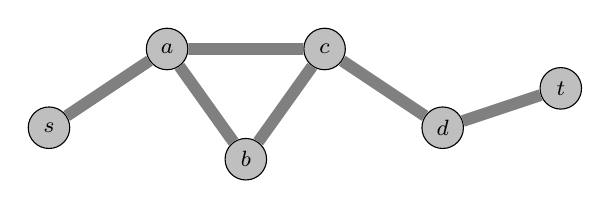
\begin{tikzpicture}
            \tikzstyle{every node}=[circle, fill=lightgray, draw=black, inner sep=2pt, minimum size=1.5em, font=\footnotesize, text=black]
            \tikzstyle{edge}=[gray, line width=1.5mm]
       
            \node (s) at (0.5,1) {$s$};
            \node (a) at (2,2) {$a$};
            \node (b) at (3,0.6) {$b$};
            \node (c) at (4,2) {$c$};
            \node (d) at (5.5,1) {$d$};
            \node (t) at (7,1.5) {$t$};
       
            \draw[edge] (s) -- (a) -- (c) -- (d) -- (t);
            \draw[edge] (a) -- (b) -- (c);
          \end{tikzpicture}
          \caption{The input graph $G$}
          \label{figure:input-graph}
    \end{subfigure}\hfill%
    \begin{subfigure}{.45\textwidth}
        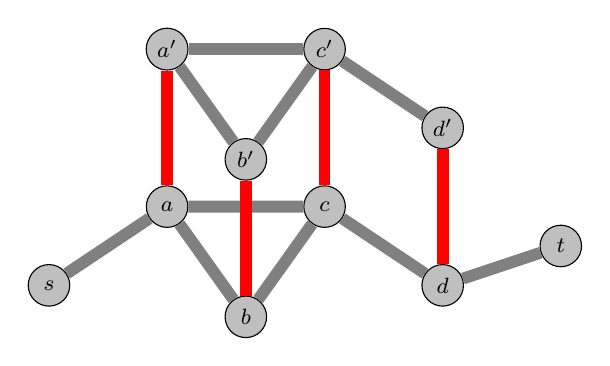
\begin{tikzpicture}
            \tikzstyle{every node}=[circle, fill=lightgray, draw=black, inner sep=2pt, minimum size=1.5em, font=\footnotesize, text=black]
            \tikzstyle{edge}=[gray, line width=1.5mm]
       
            \node (s) at (0.5,1) {$s$};
            \node (a) at (2,2) {$a$};
            \node (b) at (3,0.6) {$b$};
            \node (c) at (4,2) {$c$};
            \node (d) at (5.5,1) {$d$};
            \node (t) at (7,1.5) {$t$};

            \node (a') at (2,4) {$a'$};
            \node (b') at (3,2.6) {$b'$};
            \node (c') at (4,4) {$c'$};
            \node (d') at (5.5,3) {$d'$};
       
            \draw[edge] (s) -- (a) -- (c) -- (d) -- (t);
            \draw[edge] (a) -- (b) -- (c);

            \draw[edge] (a') -- (b') -- (c') -- (d');
            \draw[edge] (a') -- (c');

            \tikzstyle{edge}=[red, line width=1.5mm]
            \draw[edge] (a) -- (a');
            \draw[edge] (b) -- (b');
            \draw[edge] (c) -- (c');
            \draw[edge] (d) -- (d');
        \end{tikzpicture}
        \caption{The mirror graph $M$ of $G$, with the matching marked in red}
        \label{figure:mirror-graph}
    \end{subfigure}
    \caption{Reduction from \textsc{Shortest Odd Path} to \textsc{Shortest Alternating Path}.}
    \label{figure:mirror-construction}
 \end{figure}

Our reduction from \textsc{Shortest Odd Path} to \textsc{Shortest Alternating Path} follows:
\begin{enumerate}
    \item Let $(G, s, t)$ be an instance of \textsc{Shortest Odd Path}.
    \item Construct $M$ as the mirror graph of $G$, and let $F$ be the matching in $M$. Now $(M, s, t, F)$ is an instance of \textsc{Shortest Alternating Path}.
    \item Let $P'$ be the shortest alternating path of $(M, s, t, F)$, if one exists. If none exist, then we do not have any odd $s$-$t$-paths in $G$ either and are already done.
    \item Construct $P$ by filtering out the edges in the matching from $P'$, and for each edge $e' \in E(M)$ from the mirror side of $M$ we replace it by the corresponding edge $\mirror(e') \in E(G)$ from the real side.
    \label{point:translate_alternating_path}
    \item Now $P$ is the shortest odd $s$-$t$-path in $G$.
\end{enumerate}

For example, if our input $G$ for \textsc{Shortest Odd Path} is \Cref{figure:input-graph}, then $M$ and $F$ could look like \Cref{figure:mirror-graph}. The only alternating $s$-$t$-path is $P'~:= [(s,a), (a, a'), (a',b'), (b',b)$, $(b,c), (c,c'), (c',d'), (d',d), (d,t)]$. When we translate it to a path in $G$, we end up with $P~:= [(s,a),(a,b),(b,c),(c,d),(d,t)]$, which is the shortest odd $s$-$t$-path in $G$. 

Now that we have two copies of most vertices in $M$, we run the risk of accidentally using the same vertex multiple times and ending up with a walk rather than a path in $G$, like with our algorithm in \Cref{chapter:odd-walk}. The key to note here is that $F$ is an (almost) perfect matching, and when we step on a vertex $u$ we have to cross the mirror and step on $\mirror(u)$ next. We will never visit $u$, go somewhere else, and then later come back to visit $\mirror(u)$. So both copies must be used directly after each other, and when we translate the path in $M$ into a path in $G$ the two copies are effectively merged into just a single step in the path. Therefore, vertices are never repeated and we always end up with a path.

To see why the reduction necessarily yields an \emph{odd} path, simply observe that for each step we take in the graph, we have to go to the other side of the mirror. If we take another step, we get back to the same side again. It is only when we reach the target vertex $t$ that we can stop and not have to go to the other side. Therefore, to reach a neighbor of $t$, we must have used an even number of edges from the matching and an even number of edges not in the matching. When we take the last step to reach $t$ we have used an odd number of edges and thus found an odd path. If this alternating $s$-$t$-path in $M$ is the shortest such path, then the corresponding path in $G$ must also be the \emph{shortest} odd $s$-$t$-path in $G$. 

The interested reader may see \cite{source:derigs_shortest_odd_path} for more details on this reduction.

\todo{Here we should mention that SAP is NP-complete, and who proved it, and it does not matter to us.}
Ball and Derigs \cite{source:shortest_alternating_path} have shown how to efficiently solve \textsc{Shortest Alternating Path}. In their algorithms, subgraphs are shrunk into pseudonodes whenever possible, to make the graph smaller. The drawback is that certain pseudonodes must later be expanded again, which is the most complicated and expensive part of their algorithms. In our case, however, we have a special case of \textsc{Shortest Alternating Path}. The set $F$ is, except for $s$ and $t$, a perfect matching of $M$, and we will therefore never have to expand pseudonodes after shrinking them. The curious reader may visit \cite{source:shortest_alternating_path} for more on these algorithms and why our almost-perfect matching is a simpler case.

\section{The idea for our \textsc{Shortest Alternating Path} algorithm}
We will explain the general idea of our algorithm by following an example, and solve for the graph in \Cref{figure:input-graph}. First, we construct the mirror graph as explained in \Cref{subsection:reduction}, to produce the graph in \Cref{figure:mirror-graph}. Then we initialize an empty priority queue of vertices and edges to be scanned. For each vertex $u \in V(M)$, we denote
\begin{itemize}
    \item $d^+_u~:=$ the length of the shortest alternating $s$-$u$-path ending on a matched edge
    \item $d^-_u~:=$ the length of the shortest alternating $s$-$u$-path ending on a non-matched edge
    \item $\pred_u~:=$ the last edge used to find $u$'s most recent value for $d^-_u$
\end{itemize}

Initially, these are either $\infty$ or undefined, except for the source vertex $s$, where we can set $d^+_s~:= 0$. Then, for each edge $e \in N(s)$, we can set $d^-_{\too(e)}~:= \weight(e)$, $pred_{to(e)}~:= e$, and add $\too(e)$ to our priority queue with priority $2 \cdot \weight(e)$.

We visualize it in the diagram below.

\begin{minipage}{.75\linewidth}
    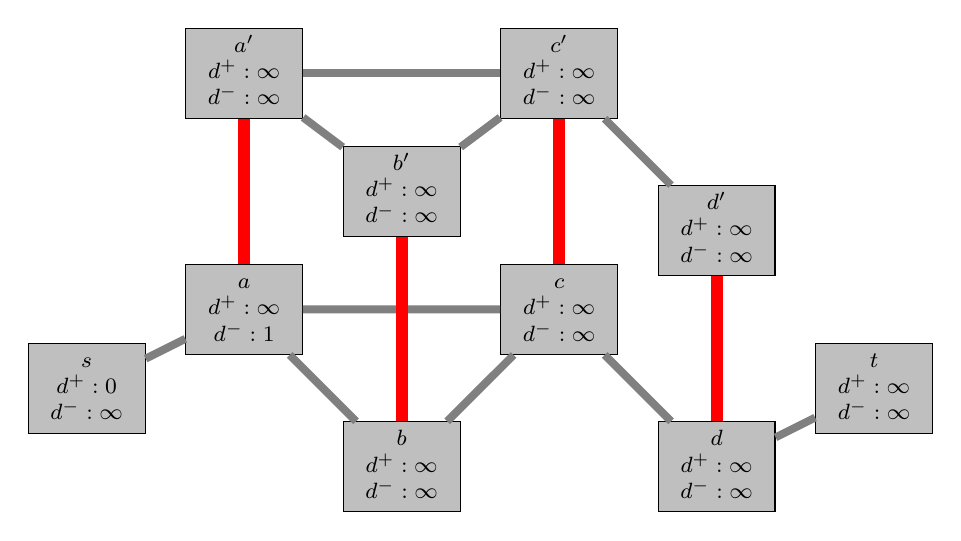
\begin{tikzpicture}{text centered}
        \tikzstyle{every node}=[rectangle, fill=lightgray, draw=black, inner sep=2pt, minimum size=1.5em, font=\footnotesize, text=black]
        \tikzstyle{edge}=[gray, line width=1mm]
   
        \node (s) at (0,1)    {\begin{tabular}{c} $s$  \\ $d^+:0$       \\ $d^-:\infty$ \end{tabular}};
        \node (a) at (2,2)    {\begin{tabular}{c} $a$  \\ $d^+:\infty$  \\ $d^-:1$      \end{tabular}};
        \node (b) at (4,0)    {\begin{tabular}{c} $b$  \\ $d^+:\infty$  \\ $d^-:\infty$ \end{tabular}};
        \node (c) at (6,2)    {\begin{tabular}{c} $c$  \\ $d^+:\infty$  \\ $d^-:\infty$ \end{tabular}};
        \node (d) at (8,0)    {\begin{tabular}{c} $d$  \\ $d^+:\infty$  \\ $d^-:\infty$ \end{tabular}};
        \node (t) at (10,1)   {\begin{tabular}{c} $t$  \\ $d^+:\infty$  \\ $d^-:\infty$ \end{tabular}};

        \node (a') at (2,5)   {\begin{tabular}{c} $a'$ \\ $d^+:\infty$  \\ $d^-:\infty$ \end{tabular}};
        \node (b') at (4,3.5) {\begin{tabular}{c} $b'$ \\ $d^+:\infty$  \\ $d^-:\infty$ \end{tabular}};
        \node (c') at (6,5)   {\begin{tabular}{c} $c'$ \\ $d^+:\infty$  \\ $d^-:\infty$ \end{tabular}};
        \node (d') at (8,3)   {\begin{tabular}{c} $d'$ \\ $d^+:\infty$  \\ $d^-:\infty$ \end{tabular}};
   
        \draw[edge] (s) -- (a) -- (c) -- (d) -- (t);
        \draw[edge] (a) -- (b) -- (c);

        \draw[edge] (a') -- (b') -- (c') -- (d');
        \draw[edge] (a') -- (c');

        \tikzstyle{edge}=[red, line width=1.5mm]
        \draw[edge] (a) -- (a');
        \draw[edge] (b) -- (b');
        \draw[edge] (c) -- (c');
        \draw[edge] (d) -- (d');
    \end{tikzpicture}
\end{minipage}\hfill%
\begin{minipage}{.22\linewidth}
    Queue:
    \begin{itemize}
        \item Vertex(2,$a$)
    \end{itemize}
\end{minipage}

The first and only vertex in the queue is $a$. We pop it, set $d^+_{a'}~:= d^-_a$, and 'scan'~$a'$. By that, we mean to look at each neighbor $e \in G[a']$, and see if our new value $d^+_{a'} + \weight(e)$ is better than the previous value $d^-_{\too(e)}$. That is the case for both~$b'$ and~$c'$, so we update their values and add them to the queue. Their priorities in the queue are equal to twice their $d^-$ values, which is $2 \cdot 2 = 4$ for both of them.

\begin{minipage}{.75\linewidth}
    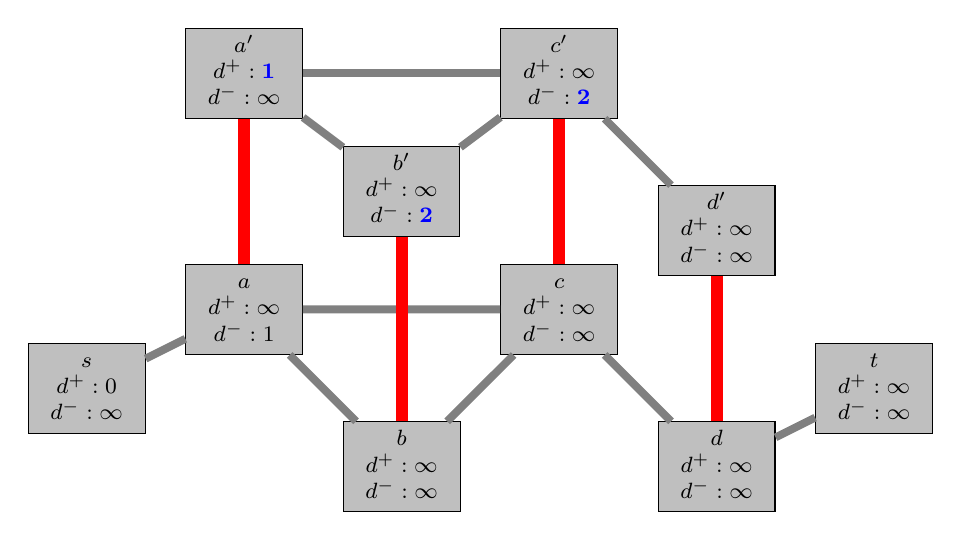
\begin{tikzpicture}{text centered}
        \tikzstyle{every node}=[rectangle, fill=lightgray, draw=black, inner sep=2pt, minimum size=1.5em, font=\footnotesize, text=black]
        \tikzstyle{edge}=[gray, line width=1mm]
   
        \node (s) at (0,1)    {\begin{tabular}{c} $s$  \\ $d^+:0$       \\ $d^-:\infty$ \end{tabular}};
        \node (a) at (2,2)    {\begin{tabular}{c} $a$  \\ $d^+:\infty$  \\ $d^-:1$      \end{tabular}};
        \node (b) at (4,0)    {\begin{tabular}{c} $b$  \\ $d^+:\infty$  \\ $d^-:\infty$ \end{tabular}};
        \node (c) at (6,2)    {\begin{tabular}{c} $c$  \\ $d^+:\infty$  \\ $d^-:\infty$ \end{tabular}};
        \node (d) at (8,0)    {\begin{tabular}{c} $d$  \\ $d^+:\infty$  \\ $d^-:\infty$ \end{tabular}};
        \node (t) at (10,1)   {\begin{tabular}{c} $t$  \\ $d^+:\infty$  \\ $d^-:\infty$ \end{tabular}};

        \node (a') at (2,5)   {\begin{tabular}{c} $a'$ \\ $d^+:\textcolor{blue}{\mathbf{1}}$       \\ $d^-:\infty$ \end{tabular}};
        \node (b') at (4,3.5) {\begin{tabular}{c} $b'$ \\ $d^+:\infty$  \\ $d^-:\textcolor{blue}{\mathbf{2}}$      \end{tabular}};
        \node (c') at (6,5)   {\begin{tabular}{c} $c'$ \\ $d^+:\infty$  \\ $d^-:\textcolor{blue}{\mathbf{2}}$      \end{tabular}};
        \node (d') at (8,3)   {\begin{tabular}{c} $d'$ \\ $d^+:\infty$  \\ $d^-:\infty$ \end{tabular}};
   
        \draw[edge] (s) -- (a) -- (c) -- (d) -- (t);
        \draw[edge] (a) -- (b) -- (c);

        \draw[edge] (a') -- (b') -- (c') -- (d');
        \draw[edge] (a') -- (c');

        \tikzstyle{edge}=[red, line width=1.5mm]
        \draw[edge] (a) -- (a');
        \draw[edge] (b) -- (b');
        \draw[edge] (c) -- (c');
        \draw[edge] (d) -- (d');
    \end{tikzpicture}
\end{minipage}\hfill%
\begin{minipage}{.26\linewidth}
    Queue:
    \begin{itemize}
        \item \st{Vertex(2,$a$)}
        \item Vertex(4,$b'$)
        \item Vertex(4,$c'$)
    \end{itemize}
\end{minipage}

The next vertex in the queue is $b'$, so we set $d^+_b~:= d^-_{b'}$ and scan $b'$:

\begin{minipage}{.75\linewidth}
    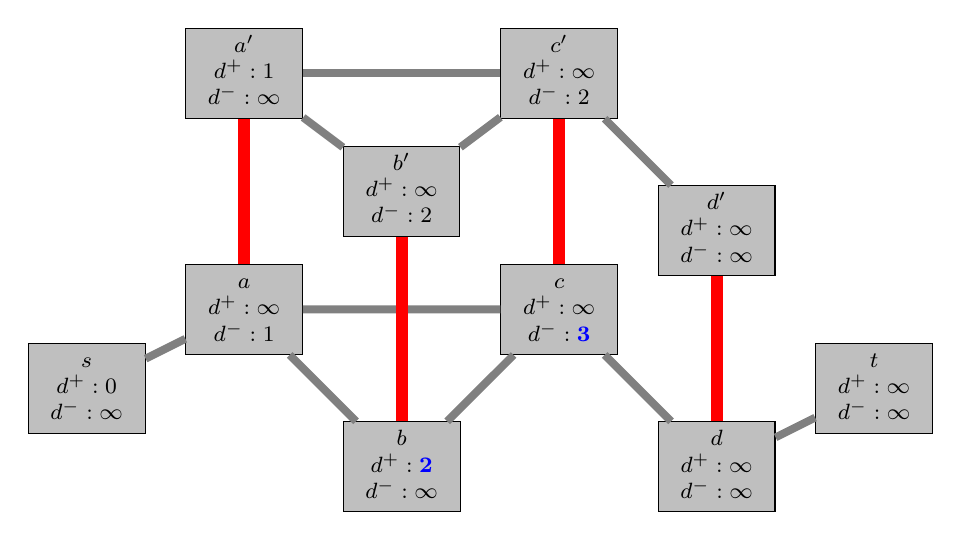
\begin{tikzpicture}{text centered}
        \tikzstyle{every node}=[rectangle, fill=lightgray, draw=black, inner sep=2pt, minimum size=1.5em, font=\footnotesize, text=black]
        \tikzstyle{edge}=[gray, line width=1mm]
   
        \node (s) at (0,1)    {\begin{tabular}{c} $s$  \\ $d^+:0$       \\ $d^-:\infty$ \end{tabular}};
        \node (a) at (2,2)    {\begin{tabular}{c} $a$  \\ $d^+:\infty$  \\ $d^-:1$      \end{tabular}};
        \node (b) at (4,0)    {\begin{tabular}{c} $b$  \\ $d^+:\textcolor{blue}{\mathbf{2}}$       \\ $d^-:\infty$ \end{tabular}};
        \node (c) at (6,2)    {\begin{tabular}{c} $c$  \\ $d^+:\infty$  \\ $d^-:\textcolor{blue}{\mathbf{3}}     $ \end{tabular}};
        \node (d) at (8,0)    {\begin{tabular}{c} $d$  \\ $d^+:\infty$  \\ $d^-:\infty$ \end{tabular}};
        \node (t) at (10,1)   {\begin{tabular}{c} $t$  \\ $d^+:\infty$  \\ $d^-:\infty$ \end{tabular}};

        \node (a') at (2,5)   {\begin{tabular}{c} $a'$ \\ $d^+:1$       \\ $d^-:\infty$ \end{tabular}};
        \node (b') at (4,3.5) {\begin{tabular}{c} $b'$ \\ $d^+:\infty$  \\ $d^-:2$      \end{tabular}};
        \node (c') at (6,5)   {\begin{tabular}{c} $c'$ \\ $d^+:\infty$  \\ $d^-:2$      \end{tabular}};
        \node (d') at (8,3)   {\begin{tabular}{c} $d'$ \\ $d^+:\infty$  \\ $d^-:\infty$ \end{tabular}};
   
        \draw[edge] (s) -- (a) -- (c) -- (d) -- (t);
        \draw[edge] (a) -- (b) -- (c);

        \draw[edge] (a') -- (b') -- (c') -- (d');
        \draw[edge] (a') -- (c');

        \tikzstyle{edge}=[red, line width=1.5mm]
        \draw[edge] (a) -- (a');
        \draw[edge] (b) -- (b');
        \draw[edge] (c) -- (c');
        \draw[edge] (d) -- (d');
    \end{tikzpicture}
\end{minipage}\hfill%
\begin{minipage}{.26\linewidth}
    Queue:
    \begin{itemize}
        \item \st{Vertex(4,$b'$)}
        \item Vertex(4,$c'$)
        \item Vertex(6,$c$)
    \end{itemize}
\end{minipage}

Now $c'$ is the next in the queue, we set $d^+_c~:= d^-c'$ and scan $c'$. This is where the interesting part happens: now we have set both $d^+$ and $d^-$ for $b$ and $c$, and that means that we have found an odd cycle in the graph. The edge between them, $e$, is called the \emph{blossom edge}, and is marked in green. We add $e$ to the queue, with the priority $d^+_c + d^+_b + \weight(e)$.

\begin{minipage}{.75\linewidth}
    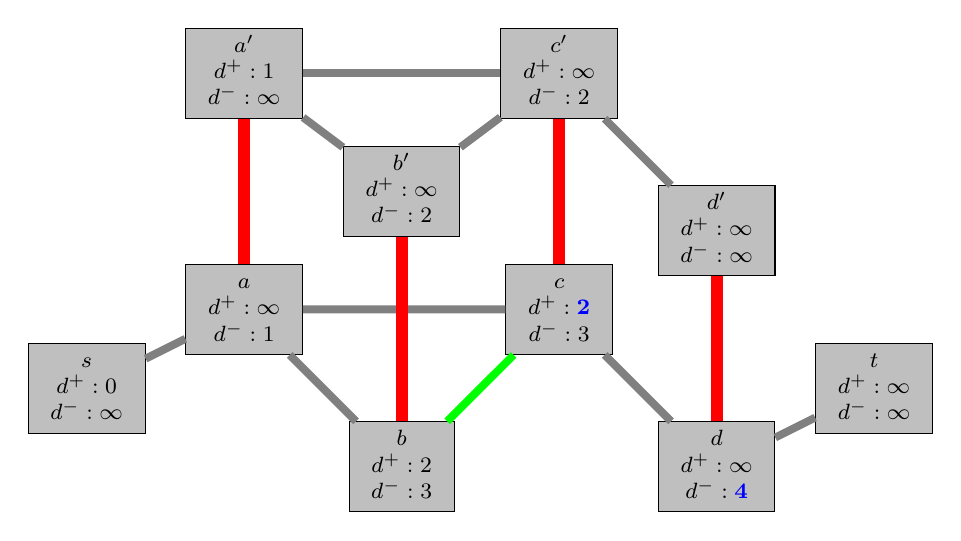
\begin{tikzpicture}{text centered}
        \tikzstyle{every node}=[rectangle, fill=lightgray, draw=black, inner sep=2pt, minimum size=1.5em, font=\footnotesize, text=black]
        \tikzstyle{edge}=[gray, line width=1mm]
   
        \node (s) at (0,1)    {\begin{tabular}{c} $s$  \\ $d^+:0$       \\ $d^-:\infty$ \end{tabular}};
        \node (a) at (2,2)    {\begin{tabular}{c} $a$  \\ $d^+:\infty$  \\ $d^-:1$      \end{tabular}};
        \node (b) at (4,0)    {\begin{tabular}{c} $b$  \\ $d^+:2$       \\ $d^-:3$      \end{tabular}};
        \node (c) at (6,2)    {\begin{tabular}{c} $c$  \\ $d^+:\textcolor{blue}{\mathbf{2}}$       \\ $d^-:3$      \end{tabular}};
        \node (d) at (8,0)    {\begin{tabular}{c} $d$  \\ $d^+:\infty$  \\ $d^-:\textcolor{blue}{\mathbf{4}}$      \end{tabular}};
        \node (t) at (10,1)   {\begin{tabular}{c} $t$  \\ $d^+:\infty$  \\ $d^-:\infty$ \end{tabular}};

        \node (a') at (2,5)   {\begin{tabular}{c} $a'$ \\ $d^+:1$       \\ $d^-:\infty$ \end{tabular}};
        \node (b') at (4,3.5) {\begin{tabular}{c} $b'$ \\ $d^+:\infty$  \\ $d^-:2$      \end{tabular}};
        \node (c') at (6,5)   {\begin{tabular}{c} $c'$ \\ $d^+:\infty$  \\ $d^-:2$      \end{tabular}};
        \node (d') at (8,3)   {\begin{tabular}{c} $d'$ \\ $d^+:\infty$  \\ $d^-:\infty$ \end{tabular}};
   
        \draw[edge] (s) -- (a) -- (c) -- (d) -- (t);
        \draw[edge] (a) -- (b);

        \draw[edge] (a') -- (b') -- (c') -- (d');
        \draw[edge] (a') -- (c');

        \tikzstyle{edge}=[red, line width=1.5mm]
        \draw[edge] (a) -- (a');
        \draw[edge] (b) -- (b');
        \draw[edge] (c) -- (c');
        \draw[edge] (d) -- (d');

        \tikzstyle{edge}=[green, line width=1mm]
        \draw[edge] (b) -- (c);
    \end{tikzpicture}
\end{minipage}\hfill%
\begin{minipage}{.26\linewidth}
    Queue:
    \begin{itemize}
        \item \st{Vertex(4,$c'$)}
        \item Blossom(5,($b$,$c$))
        \item Vertex(6,$c$)
        \item Vertex(6,$d$)
    \end{itemize}
\end{minipage}

Next up is to scan this blossom edge, and compute its corresponding odd cycle by backtracking from $c$ and $b$ until they meet at $a'$. To visualize the cycle, we like to 'stretch out' the graph a little, and draw it like below. Note that some of the edges are omitted for clarity. Now we can see that the cycle consists of [$a',c',c,b,b',a'$]. We call the set $\mathbb{B}~:= \{c',c,b,b'\}$ a \emph{blossom}, and $a'$ the \emph{base} of the blossom, inspired by the famous Blossom algorithm by \cite{source:blossom}.

\begin{minipage}{.7\linewidth}
    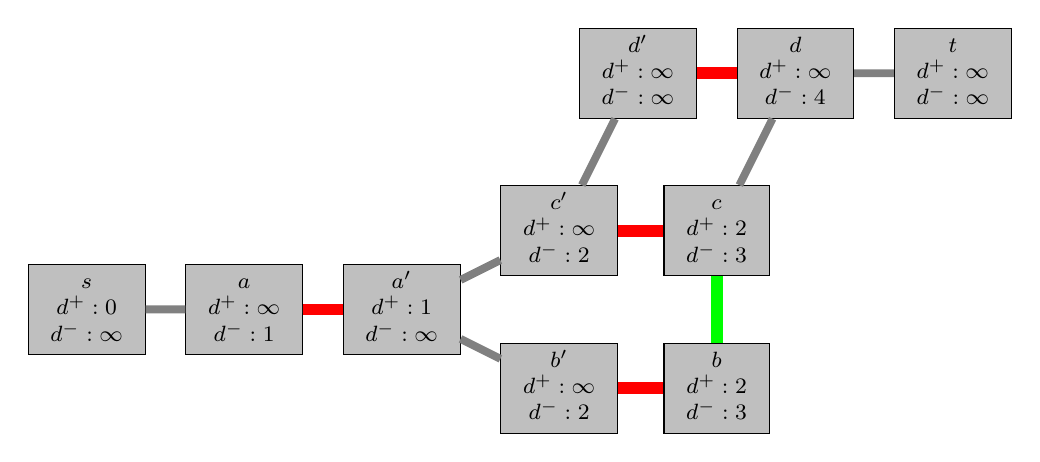
\begin{tikzpicture}{text centered}
        \tikzstyle{every node}=[rectangle, fill=lightgray, draw=black, inner sep=2pt, minimum size=1.5em, font=\footnotesize, text=black]
        \tikzstyle{edge}=[gray, line width=1mm]
   
        \node (s) at (0,1)    {\begin{tabular}{c} $s$  \\ $d^+:0$       \\ $d^-:\infty$ \end{tabular}};
        \node (a) at (2,1)    {\begin{tabular}{c} $a$  \\ $d^+:\infty$  \\ $d^-:1$      \end{tabular}};
        \node (b) at (8,0)    {\begin{tabular}{c} $b$  \\ $d^+:2$       \\ $d^-:3$      \end{tabular}};
        \node (c) at (8,2)    {\begin{tabular}{c} $c$  \\ $d^+:2$       \\ $d^-:3$      \end{tabular}};
        \node (d) at (9,4)    {\begin{tabular}{c} $d$  \\ $d^+:\infty$  \\ $d^-:4$      \end{tabular}};
        \node (t) at (11,4)   {\begin{tabular}{c} $t$  \\ $d^+:\infty$  \\ $d^-:\infty$ \end{tabular}};

        \node (a') at (4,1)   {\begin{tabular}{c} $a'$ \\ $d^+:1$       \\ $d^-:\infty$ \end{tabular}};
        \node (b') at (6,0)   {\begin{tabular}{c} $b'$ \\ $d^+:\infty$  \\ $d^-:2$      \end{tabular}};
        \node (c') at (6,2)   {\begin{tabular}{c} $c'$ \\ $d^+:\infty$  \\ $d^-:2$      \end{tabular}};
        \node (d') at (7,4)   {\begin{tabular}{c} $d'$ \\ $d^+:\infty$  \\ $d^-:\infty$ \end{tabular}};
   
        \draw[edge] (s) -- (a) -- (a') -- (c') -- (d');
        \draw[edge] (a') -- (b');
        \draw[edge] (c) -- (d) -- (t);

        \tikzstyle{edge}=[red, line width=1.5mm]
        \draw[edge] (a) -- (a');
        \draw[edge] (b) -- (b');
        \draw[edge] (c) -- (c');
        \draw[edge] (d) -- (d');

        \tikzstyle{edge}=[green, line width=1.5mm]
        \draw[edge] (b) -- (c);
    \end{tikzpicture}
\end{minipage}\hfill%
\begin{minipage}{.26\linewidth}
    \vspace{2cm}
    Queue:
    \begin{itemize}
        \item Blossom(5,($b$,$c$))
        \item Vertex(6,$c$)
        \item Vertex(6,$d$)
    \end{itemize}
\end{minipage}

The first reason why we care about this blossom is because now we can immediately set the final, optimal $d^-$ and $d^+$ for all the vertices in the blossom. That is because we now have two alternating paths to each vertex, one goes around the cycle while the other takes the shortcut. One of these ends up on a matched edge, and the other on a normal edge. Furthermore, both of these are the optimal paths and can be used to set final values for $d^+$ and $d^-$. For example, to go from $s$ to $c'$, we can either go through [$s,a,a',c'$] with a cost of $d^-_c$, or go along [$s,a,a',b',b,c,c'$] with a cost of $d^+_c$.

More specifically, for each $u \in \mathbb{B}$: \begin{itemize}
    \item If $d^+_u = \infty$, we set $d^+_u = d^-_{\mirror(u)}$.
    \item If we can improve $d^-_u$ by coming from its neighbor in the blossom, we do so.
\end{itemize}
After all these values have been set, we immediately scan all the vertices in $\mathbb{B}$ that just received values for $d^+$. In this example, we scan $c'$ and $b'$, and discover $d'$. Unfortunately, since this is a very small blossom we don't have any vertices that receive new values for $d^-$.

\begin{minipage}{.7\linewidth}
    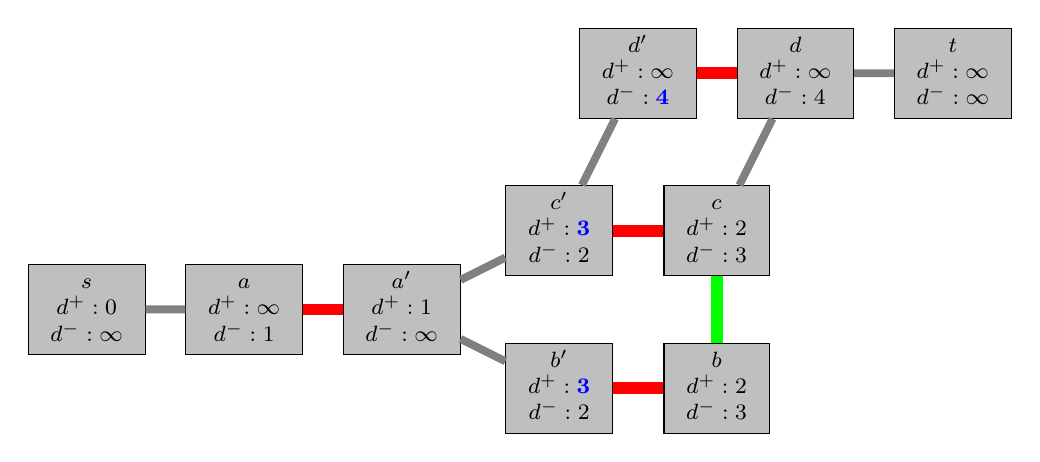
\begin{tikzpicture}{text centered}
        \tikzstyle{every node}=[rectangle, fill=lightgray, draw=black, inner sep=2pt, minimum size=1.5em, font=\footnotesize, text=black]
        \tikzstyle{edge}=[gray, line width=1mm]
   
        \node (s) at (0,1)    {\begin{tabular}{c} $s$  \\ $d^+:0$       \\ $d^-:\infty$ \end{tabular}};
        \node (a) at (2,1)    {\begin{tabular}{c} $a$  \\ $d^+:\infty$  \\ $d^-:1$      \end{tabular}};
        \node (b) at (8,0)    {\begin{tabular}{c} $b$  \\ $d^+:2$       \\ $d^-:3$      \end{tabular}};
        \node (c) at (8,2)    {\begin{tabular}{c} $c$  \\ $d^+:2$       \\ $d^-:3$      \end{tabular}};
        \node (d) at (9,4)    {\begin{tabular}{c} $d$  \\ $d^+:\infty$  \\ $d^-:4$      \end{tabular}};
        \node (t) at (11,4)   {\begin{tabular}{c} $t$  \\ $d^+:\infty$  \\ $d^-:\infty$ \end{tabular}};

        \node (a') at (4,1)   {\begin{tabular}{c} $a'$ \\ $d^+:1$       \\ $d^-:\infty$ \end{tabular}};
        \node (b') at (6,0)   {\begin{tabular}{c} $b'$ \\ $d^+:\textcolor{blue}{\mathbf{3}}$       \\ $d^-:2$      \end{tabular}};
        \node (c') at (6,2)   {\begin{tabular}{c} $c'$ \\ $d^+:\textcolor{blue}{\mathbf{3}}$       \\ $d^-:2$      \end{tabular}};
        \node (d') at (7,4)   {\begin{tabular}{c} $d'$ \\ $d^+:\infty$  \\ $d^-:\textcolor{blue}{\mathbf{4}}$      \end{tabular}};
   
        \draw[edge] (s) -- (a) -- (a') -- (c') -- (d');
        \draw[edge] (a') -- (b');
        \draw[edge] (c) -- (d) -- (t);

        \tikzstyle{edge}=[red, line width=1.5mm]
        \draw[edge] (a) -- (a');
        \draw[edge] (b) -- (b');
        \draw[edge] (c) -- (c');
        \draw[edge] (d) -- (d');

        \tikzstyle{edge}=[green, line width=1.5mm]
        \draw[edge] (b) -- (c);
    \end{tikzpicture}
\end{minipage}\hfill%
\begin{minipage}{.26\linewidth}
    \vspace{2cm}
    Queue:
    \begin{itemize}
        \item \st{Blossom(5,($b$,$c$))}
        \item Vertex(6,$c$)
        \item Vertex(6,$d$)
        \item Vertex(8,$d'$)
    \end{itemize}
\end{minipage}

The second reason we compute the blossom is that we no longer care much about the individual vertices in $\mathbb{B}$, and can shrink it into just the base $a'$. We will still scan vertices like $c$ from the queue as before, but whenever we are backtracking to compute blossoms we can skip the vertices in $\mathbb{B}$ entirely and go straight to the base $a'$ instead. In this example, in a few iterations, the algorithm will find either $(d',a')$ or $(d,a')$ as a blossom edge, with just $\{d,d'\}$ as its blossom and $a'$ as the base here as well. If we didn't contract the previous blossom, this new blossom would instead consist of $\{c',c,b,b',d,d'\}$, but we are already completely done with most of those vertices and computing all of it again would be a waste. Therefore we shrink them. 

If the concerned reader is familiar with the more general \textsc{Shortest Alternating Path} algorithm \cite{source:shortest_alternating_path} or the original blossom algorithm \cite{source:blossom}, and worry that such pseudonodes often have to be expanded again, then remember that in our case the set $F$ is an almost-perfect matching and those cases never happen. \todo{trenger vi si dette? Droppe det? Formulere det annerledes?}

\begin{minipage}{.7\linewidth}
    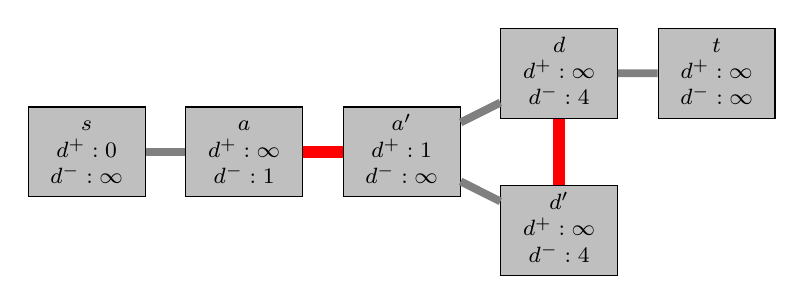
\begin{tikzpicture}{text centered}
        \tikzstyle{every node}=[rectangle, fill=lightgray, draw=black, inner sep=2pt, minimum size=1.5em, font=\footnotesize, text=black]
        \tikzstyle{edge}=[gray, line width=1mm]
   
        \node (s)  at (0,1) {\begin{tabular}{c} $s$  \\ $d^+:0$       \\ $d^-:\infty$ \end{tabular}};
        \node (a)  at (2,1) {\begin{tabular}{c} $a$  \\ $d^+:\infty$  \\ $d^-:1$      \end{tabular}};
        \node (a') at (4,1) {\begin{tabular}{c} $a'$ \\ $d^+:1$       \\ $d^-:\infty$ \end{tabular}};
        \node (d)  at (6,2) {\begin{tabular}{c} $d$  \\ $d^+:\infty$  \\ $d^-:4$      \end{tabular}};
        \node (d') at (6,0) {\begin{tabular}{c} $d'$ \\ $d^+:\infty$  \\ $d^-:4$      \end{tabular}};
        \node (t)  at (8,2) {\begin{tabular}{c} $t$  \\ $d^+:\infty$  \\ $d^-:\infty$ \end{tabular}};
        
        \draw[edge] (s) -- (a);
        \draw[edge] (a') -- (d) -- (t);
        \draw[edge] (a') -- (d');

        \tikzstyle{edge}=[red, line width=1.5mm]
        \draw[edge] (a) -- (a');
        \draw[edge] (d) -- (d');
    \end{tikzpicture}
\end{minipage}\hfill%
\begin{minipage}{.26\linewidth}
    \vspace{2cm}
    Queue:
    \begin{itemize}
        \item Vertex(6,$c$)
        \item Vertex(6,$d$)
        \item Vertex(8,$d'$)
    \end{itemize}
\end{minipage}

Let us now skip a few steps, until $t$ eventually reaches the front of the queue. At that point, we have that $d^-_t = 5$, and that is also the cost of the shortest odd path in our original input graph. To compute the exact path we can backtrack from $t$ to $s$ and then translate that path as described in Step \ref{point:translate_alternating_path} of our reduction in \Cref{subsection:reduction}. We end up with the path [$(s,a),(a,b),(b,c),(c,d),(d,t)$], which is the shortest odd $s$-$t$-path in the graph.

\todo[inline]{Would be nice with a figure of a larger blossom, to better show what the structure is, and how those values are set.}